%arara : pdflatex
\documentclass[•]{article}

\usepackage{../../TP0/style}

\begin{document}
\def\reportnumber{1}
\def\reporttitle{Mesure du temps d'exécution d'un programme.}
%----------------------------------------------------------------------------------------
%	TITLE PAGE
%----------------------------------------------------------------------------------------


\begin{titlepage} % Suppresses displaying the page number on the title page and the subsequent page counts as page 1
	\newcommand{\HRule}{\rule{\linewidth}{0.5mm}} % Defines a new command for horizontal lines, change thickness here
	
	\center % Centre everything on the page
	
	%------------------------------------------------
	%	Headings
	%------------------------------------------------
	
	\baselineskip=2\baselineskip 
	\textsc{\LARGE Université des Sciences et de la Technologie Houari Boumediene}%\\[1cm] % Main heading such as the name of your university/college

	%------------------------------------------------
	%	Logo
	%------------------------------------------------
	
	%\vfill\vfill
	\vfill
	
\includegraphics[width=0.3\textwidth]{../style/USTHB_Logo.png}\\[1cm] % Include a department/university logo - this will require the graphicx package
	 
	%----------------------------------------------------------------------------------------
	
	\textsc{\Large Compilation}\\[0.5cm] % Major heading such as course name
	%\textsc{\large Minor Heading}\\[0.5cm] % Minor heading such as course title
	
	%------------------------------------------------
	%	Title
	%------------------------------------------------
	
	\HRule\\[0.4cm]
	\baselineskip=1.2\baselineskip 
	{\huge\bfseries Rapport de Projet \\
	 \reporttitle}\\[0.4cm] % Title of your document
	
	\HRule\\[1.5cm]
	
	%------------------------------------------------
	%	Author(s)
	%------------------------------------------------
	
	\begin{minipage}{0.4\textwidth}
		\begin{flushleft}
			\large
			\textit{Binôme: groupe 4}\\
			HOUACINE  \textsc{Naila Aziza} % Your name
			\\
			MOHAMMEDI \textsc{Haroune } % Your name
			
		\end{flushleft}
	\end{minipage}
	~
	\begin{minipage}{0.4\textwidth}
		\begin{flushright}
			\large
			\textit{Professeur}\\
			Mme. MEKAHLIA \textsc{Fatma Zohra} % Supervisor's name
		\end{flushright}
	\end{minipage}
	
	%------------------------------------------------
	%	Date
	%------------------------------------------------
	
	\vfill\vfill\vfill % Position the date 3/4 down the remaining page
	
	{\large\today} % Date, change the \today to a set date if you want to be precise
	
	
	\vfill % Push the date up 1/4 of the remaining page
	
\end{titlepage}


\section{Partie I: Développement de l'algorithme et du programme pour le problème du calcul de la somme des n premiers nombres entiers naturels.}

\subsection{Développement de l'algorithme itératif qui permet de calculer la somme S des n premiers nombres entiers naturels.}
\textrm{L'écriture de ces algorithme sera accompagné de commentaire représentant le nombre de mot mémoire que prend chaque instruction puis celui de tous l'algorithme.}  

\subsubsection{En utilisant la forme "pour ... faire":}
\textrm{L'algorithme développé ci\-dessous, nommé Algorithme\_Somme\_Iteratif\_pour, utilise la forme de répétition : Pour ... faire ... fait.}
\begin{sql}

 Algorithme_Somme_Iteratif_pour
 
 VAR
 i,N,S : entier;				//3 mots mémoire
 
 Debut
	ecrire("Donner N = ");		//1 mot mémoire
	lire(N);					//1 mot mémoire
	
	S = 0;						//1 mot mémoire
	
	pour(i=1 ; i <= N ; i++)	//4 mots mémoire
	  faire
		S = S + i;				//2 mots mémoire
	  fait;
	  
	ecrire("La somme = ",S);	//1 mot mémoire
	
 Fin.
\end{sql}
\textrm{Totale de mots mémoire = 13 MM}

\subsubsection{En utilisant la forme "tant que ... faire":}
\textrm{L algorithme développé ci\-dessous, nommé Algorithme\_Somme\_Iteratif\_tant\_que, utilise la forme de répétition : tant que ... faire ... fait.}
\begin{sql}

 Algorithme_Somme_Iteratif_tant_que
 
 VAR
 i,N,S : entier;				//3 mots mémoire
 
 Debut
	ecrire("Donner N = ");		//1 mot mémoire
	lire(N);					//1 mot mémoire
	
	S = 0;						//1 mot mémoire
	i = 1;						//1 mot mémoire
	
	tant que(i <= N)			//1 mot mémoire
	  faire
		S = S + i;				//2 mots mémoire
		i = i + 1;				//2 mots mémoire
	  fait;
	  
	ecrire("La somme = ",S);	//1 mot mémoire
	
 Fin.
\end{sql}
\textrm{Totale de mots mémoire = 13 MM}

\subsubsection{En utilisant la forme "répéter ... jusqu'à":}
\textrm{L algorithme développé ci\-dessous, nommé Algorithme\_Somme\_Iteratif\_répéter\_jusqu\_a, utilise la forme de répétition : répéter ... jusqu'à ...}
\begin{sql}

 Algorithme_Somme_Iteratif_répéter_jusqu_a
 
 VAR
 i,N,S : entier;				//3 mots mémoire
 
 Debut
	ecrire("Donner N = ");		//1 mot mémoire
	lire(N);					//1 mot mémoire
	
	S = 0;						//1 mot mémoire
	i = 1;						//1 mot mémoire
	
	répéter
		S = S + i;				//2 mots mémoire
		i = i + 1;				//2 mots mémoire
	  jusqu a(i > N);			//1 mot mémoire
	  
	ecrire("La somme = ",S);	//1 mot mémoire
	
 Fin.
\end{sql}
\textrm{Totale de mots mémoire = 13 MM}

\subsection{Développement des programmes itératifs en langage C.}
\subsubsection{En utilisant la forme "FOR":}
\begin{sql}
 #include<stdio.h>
 #include<stdlib.h> 
 
 int main()
 {
	long int i,N,S;
	
	printf("Donner N = ");
	scanf("%Ld",&N);
	
	S=0;
	
	for(i=1 ; i <= N ; i++)
	{
		S = S + i;
	}
	
	printf("La somme S = %Ld",S);
	return 0;
 }
\end{sql}

\subsubsection{En utilisant la forme "WHILE":}
\begin{sql}
 #include<stdio.h>
 #include<stdlib.h>
 
 int main()
 {
	long int i,N,S;
	
	printf("Donner N = ");
	scanf("%Ld",&N);
	
	S=0; i=1;
	
	while(i <= N)
	{
		S = S + i;
		i = i + 1;
	}
	
	printf("La somme S = %Ld",S);
	return 0;
 }
\end{sql}

\subsubsection{En utilisant la forme "DO ... WHILE":}
\begin{sql}
 #include<stdio.h>
 #include<stdlib.h>
 
 int main()
 {
	long int i,N,S;
	
	printf("Donner N = ");
	scanf("%Ld",&N);
	
	S=0; i=1;
	
	Do
	{
		S = S + i;
		i = i + 1;
	}while(i > N)
	
	printf("La somme S = %Ld",S);
	return 0;
 }
\end{sql}
\textrm{ }
\\

\subsection{Développement de l'algorithme récursif pour le problème.}

\begin{sql}
Procedure_Somme_Récursif(N , S : entier)
 
 VAR
 
 Debut									
 
	Si( N <= 0)										//1 mot mémoire
		Alors ecrire("La Somme S = ",S);			//1 mot mémoire
		Sinon   S = S + N;							//2 mots mémoire
				Algorithme_Somme_Récursif(N - 1,S);	//2 mots mémoire
	FinSi;
	
 Fin.
 
 
 Algorithme_Somme_Récursif()
 
 VAR
 
 Debut
	N: entier;										//1 mot mémoire

    ecrire("Donner N = ");							//1 mot mémoire
	lire(N);										//1 mot mémoire

	Procedure_Somme_Récursif(N , 0);				//1 mot mémoire
 Fin.
\end{sql}
\textrm{Totale de mots mémoire = 13 MM}

\subsection{Développement du programme récursif en langage C.}
\begin{sql}
 #include<stdio.h>
 #include<stdlib.h>

 void SommeRecursive(long int N,long int S)
 {
	if(N <= 0)
	{
		printf("La somme S = %Ld \n",S);
	}else
	{
		S = S + N;
		SommeRecursive(N - 1,S);
	}
 }


int main()
{
    long int N;

    printf("Donner N = ");
	scanf("%Ld",&N);

	SommeRecursive(N,0);

	return 0;
}

\end{sql}



\textrm{  }
\\

\section{Partie II: Mesure du temps d'exécution.}
\textrm{
Pour la mesure du temps en langage C nous aurons besoin des fonctions de la gestion du temps que l'on retrouve dans la bibliothèque time.h.}

\textrm{Donc nous devant d'abord inclure la directive \#include <time.h>
Puis définir deux(2) variables notées début et fin de type clock\_t.}

\textrm{A l'aide de la fonction "clock()" :
Récupéré le Temps avant l'exécution du programme dans début et
récupéré le Temps après la fin de l'exécution du programme dans fin.}
\textrm{Calculer la différence entre début et fin dans un variable nommé : Delta de type double.} 
\textrm{Afin que le temps d'exécution Delta soit donné en secondes, nous divisons ce dernier par le paramètre CLOCKS\_PER\_SEC.}

\subsection{Mesure des temps d'exécution et Représentation par un graph}
\subsubsection{L'algorithme itératif avec boucle do while}
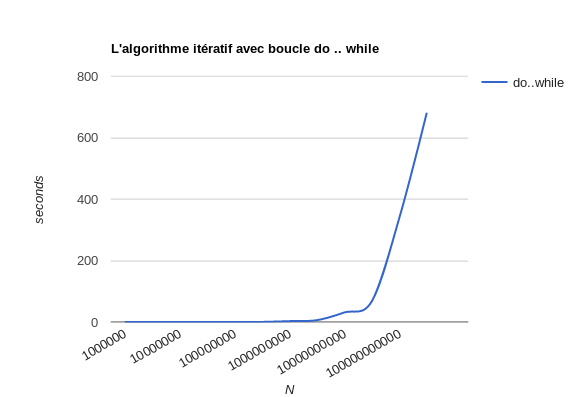
\includegraphics[width=0.75\textwidth]{dowhile.png}
\subsubsection{L'algorithme itératif avec boucle while}
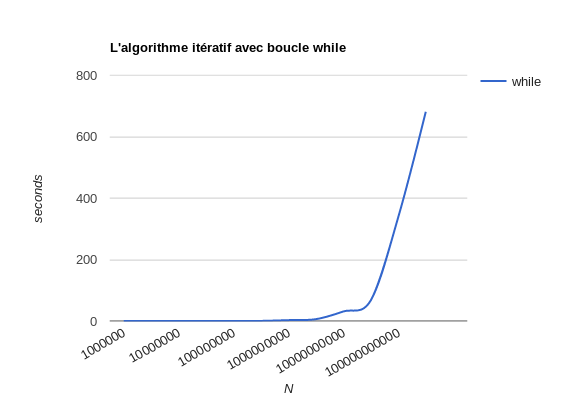
\includegraphics[width=0.75\textwidth]{while.png}
\subsubsection{L'algorithme itératif avec boucle for}
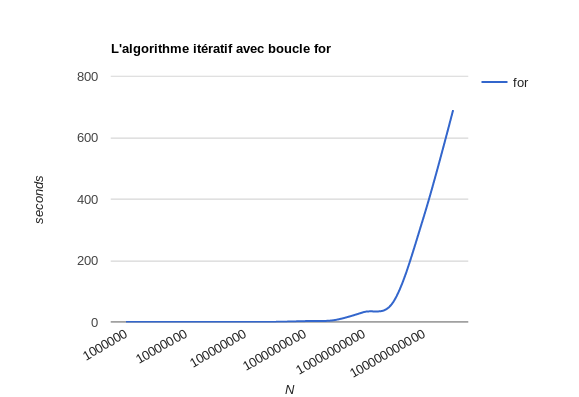
\includegraphics[width=0.75\textwidth]{for.png}
\subsection{Déduction du temps d'exécution moyen}
A partir des graphes rélaisés dans la question précédente, on peut clairement dédurie que le temps d'exécution est linéaire avec le nombre N.
\end{document}
